% 英文校正から返ってきたもの(をさらに自力で修正したもの)
% (をさらに先生に見ていただいたもの)(をさらに少し修正したもの)
% (の査読通過後に修正したもの)

% コンパイルは latexmk -lualatex -interaction=nonstopmode -halt-on-error main.tex

%
\documentclass[runningheads]{llncs}
%
\usepackage{iftex}
\ifLuaTeX
  \usepackage{fontspec}
  \usepackage{luatexja}
  \usepackage{luatexja-fontspec}
  \setmainjfont{HaranoAjiMincho}
  \setsansjfont{HaranoAjiGothic}
\else
  \usepackage[T1]{fontenc}
\fi
% T1 fonts will be used to generate the final print and online PDFs,
% so please use T1 fonts in your manuscript whenever possible.
% Other font encondings may result in incorrect characters.
%
\usepackage{graphicx}
\graphicspath{{image/}}
% Used for displaying a sample figure. If possible, figure files should
% be included in EPS format.
%
% If you use the hyperref package, please uncomment the following two lines
% to display URLs in blue roman font according to Springer's eBook style:
%\usepackage{color}
%\renewcommand\UrlFont{\color{blue}\rmfamily}
%\urlstyle{rm}
%
\usepackage{amsmath}
\usepackage{amssymb}
\usepackage{hyperref}
\hypersetup{
    colorlinks=false, 
    hidelinks         
}
\begin{document}
%
%
\title{Algorithmic Collusion in Inventory-Constrained Markets under Time-Varying Demand Scale}
%
\titlerunning{Algorithmic Collusion under Time-Varying Market}
% If the paper title is too long for the running head, you can set
% an abbreviated paper title here
%
\author{Yuzuru Kitamura\and
Katsuhide Fujita\orcidID{0000-0001-7867-4281}}
%
\authorrunning{Y. Kitamura and K. Fujita}
% First names are abbreviated in the running head.
% If there are more than two authors, 'et al.' is used.
%
\institute{Faculty of Engineering, Tokyo University of Agriculture and Technology, Japan
\email{\{kitamura,fujita\}@katfuji.lab.tuat.ac.jp}}
%\url{https://katfuji.lab.tuat.ac.jp/}}
\maketitle              % typeset the header of the contribution

% erase page number
\thispagestyle{empty} % 1ページ目のページ番号を消去
\pagestyle{empty}  

%
\begin{abstract}
Pricing systems in which agents actively learn pricing strategies for products and services are increasingly being deployed. Simulation studies have shown that the autonomy of such agents can sustain price increases across competing firms without explicit communication, a phenomenon known as algorithmic collusion. Prior work on inventory-constrained pricing markets has typically assumed that demand scale remains constant over time. In this paper, we study a more realistic setting by introducing a market environment in which demand scale varies over time and examining how this affects algorithmic collusion. Our framework preserves computable competitive and collusive benchmarks, enabling numerical comparison across demand scenarios. In experiments with Proximal Policy Optimization (PPO), we observe a negative correlation between the rate of change in demand scale and the resulting collusion index. These findings suggest that the temporal structure of demand may play an important role in the emergence of collusive behavior among learning agents.

\keywords{algorithmic collusion \and reinforcement learning \and inventory-constrained markets \and time-varying demand scale \and PPO}
% keywords{First keyword  \and Second keyword \and Another keyword.}
\end{abstract}
%
%
\section{Introduction}
Pricing algorithms are increasingly used in dynamic pricing and have attracted growing attention as firms rely more on data-driven pricing systems\cite{Chen2016}. At the same time, their autonomy has raised concerns that competing firms may sustain supra-competitive prices without explicit communication, giving rise to algorithmic collusion and related challenges for consumer welfare and competition policy\cite{mehra2016,ezrachi2017,harrington2019}.

Prior research has shown that reinforcement-learning agents can endogenously develop coordinated pricing behavior in competitive environments\cite{calvano2020a}, and this line of work has been extended to questions of institutional design and welfare\cite{johnson2020}. In particular, Friedrich et al.\cite{friedrich2025learning} studied finite-horizon, inventory-constrained episodic markets, but assumed that the demand-scale factor remains constant throughout the episode.

In many reservation markets, however, demand scale evolves over time, which may affect firms' pricing incentives and the sustainability of collusion. This paper makes two main contributions. First, we extend the inventory-constrained episodic market model by replacing the constant demand-scale factor $\lambda$ with a time-dependent factor $\lambda_t$. This extension preserves common competitive and collusive benchmarks that remain computable within practical time limits, enabling numerical comparison across demand scenarios. Second, using this framework, we examine how temporal demand variation affects algorithmic collusion. Our results show that sharper changes in demand scale are associated with a lower converged collusion index, especially under PPO, whereas DQN is less sensitive to this variation. These findings suggest that temporal demand structure can materially affect the pricing behavior learned by algorithms.

% 本論文の構成は以下の通りである．まず第2節で関連研究を概観し，第3節で在庫制約つきエピソディック市場の問題設定を与える．第4節で市場規模係数を時変化させた環境設定を述べ，第5節で固定市場規模と時変市場規模における学習結果と比較・分析を示す．最後に第6節で結論と今後の課題を述べる．


\section{Related Work}

In repeated pricing games, Q-learning-based pricing algorithms have been shown to converge to supra-competitive prices even without explicit communication among firms\cite{calvano2020a,klein2021}.
In particular, Calvano et al.\cite{calvano2020a} reported that collusive strategies supported by finite punishment phases can arise endogenously in a standard repeated Bertrand oligopoly.
The implications of such algorithmic pricing for competition law and policy have also been discussed from the perspectives of both survey work and institutional design\cite{calvano2020b,harrington2019}.

Much of this literature adopts repeated Bertrand competition as the basic environment, in which firms repeatedly choose the price of a single product using independent pricing algorithms\cite{calvano2020a,klein2021}.
As a deep-reinforcement-learning extension, Hettich\cite{hettich2021} introduced DQN\cite{mnih2015}, providing a framework that can handle larger state spaces than tabular Q-learning.
More recent work has also analyzed collusive pricing and differences in its degree in deep-reinforcement-learning-based pricing games using PPO, DQN, and related methods\cite{Schlechtinger2024,deng2024algorithmic}.
There are also studies on continuous pricing with policy-gradient methods\cite{martello2022autonomous}, as well as work that analyzes the competitive effects of pricing algorithms from both empirical and theoretical perspectives\cite{brown2021,assad2020,Abada2020,Sanchez-Cartas2022}.
Most of these studies observe only the prices determined by algorithms, whereas many real markets are subject to inventory constraints.
Friedrich et al.\cite{friedrich2025learning} showed that when learning algorithms observe both prices and inventories across repeated episodes, they can experimentally acquire collusive behavior in finite-horizon inventory-constrained markets.
% 同研究では在庫制約つきの有限期間価格競争を，有限期間マルコフゲームとして定式化し，エージェントの暗黙的共謀を分析した．各時刻で企業は価格を同時に選択し，需要に応じて販売が発生し，在庫が更新される．
Shintani et al.\cite{ShintaniUmeno2023ABCDEF} analyzed the temporal structure of average booking curves in reservation markets using real booking data from the hotel and rental-car industries.
Here, an average booking curve denotes the average cumulative number of bookings as a function of the remaining time $t$ until the deadline, aggregated across booking curves from multiple dates.
They showed that the average booking curve can be approximated by the exponential form $E[X(t)] \simeq A\exp(-\beta t)$ and referred to this regularity as the ABCDEF (Average Booking Curves Draw Exponential Functions) law.

Ito et al.\cite{ItoEtAl2024ReservationTiming} further analyzed booking timing and the temporal change in cancellation probabilities using hotel-booking data from a Japanese online travel agent (OTA), and showed that these patterns can be represented as sums of exponential functions of the days until stay and the elapsed days after booking.

\section{Problem Statement}
\label{sec:problem_statement}

Based on the setting of Friedrich et al.\cite{friedrich2025learning}, we formulate price competition in a finite-horizon (episodic), inventory-constrained market.

\subsection{Formulation as an Episodic Markov Game}
We model the market interaction as a multi-agent decision problem consisting of episodes of length $T$ (the selling horizon).
At each time step $t=1,\dots,T$ within an episode, firms (agents) simultaneously choose prices, after which demand, sales, and inventories are updated and profits are given as rewards.

We represent this setting as an episodic Markov game
$(\mathcal{S}, \mathcal{A}, P, \{R_i\}_{i=1}^N, T)$
with $N$ firms.
Here, $\mathcal{S}$ is the state space, $\mathcal{A}=\mathcal{A}_1\times\cdots\times\mathcal{A}_N$ is the joint action space of simultaneous pricing actions, $P$ is the state-transition function, and $R_i$ is the reward (profit) of firm $i$.
At each time step, firm $i$ observes the state and chooses a price action according to its policy $\pi_i$.
% 有限期間市場ではエピソード終端までの残り時間に応じて最適な価格戦略が変化し得るため，本研究では現在時刻$t$を状態に含めることで，方策がエピソード内の時間位置に条件づけられるようにする．

\subsection{Market Model: Prices, Sales, Inventory, and Rewards}
Each firm $i\in\{1,\dots,N\}$ simultaneously posts a price $p_{i,t}\ge 0$ at each time step $t$.
Each firm has a maximum quantity it can sell over the entire episode, that is, an initial inventory $I_i\in\mathbb{N}$, and we denote the remaining inventory at time $t$ by $I_{i,t}\in\{0,1,\dots,I_i\}$.
Let $p_t=(p_{1,t},\dots,p_{N,t})$ denote the price vector and $I_t=(I_{1,t},\dots,I_{N,t})$ the inventory vector.

The state consists of the previous prices, the current inventory, and the current time step, written as $s_t = (p_{t-1}, I_t, t)$.
% これは，直前の価格が競争・協調いずれの戦略にとっても重要な情報となり得ることに加え，有限期間市場ではエピソード終盤に近づくほど逸脱や懲罰の誘因が変化するため，現在時刻も戦略決定に重要な情報となり得ることを踏まえた選択である．
At $t=1$, however, $p_0$ is given exogenously as the initial price vector.

Once prices are set at each time step, demand is realized and sales are capped by the available inventory.
Let $x_{i,t}$ denote the sales quantity and $d_{i,t}$ the demand quantity (the integer demand before imposing the inventory constraint):
\begin{equation}
x_{i,t}=\min\{d_{i,t}, I_{i,t}\},
\qquad
I_{i,t+1}=I_{i,t}-x_{i,t}
\label{eq:inventory_update}
\end{equation}
The inventory is updated according to the above equation.
The reward (profit) of each firm is defined using the unit cost $c_i$ as
\begin{equation}
R_{i,t} = (p_{i,t}-c_i)\,x_{i,t}
\label{eq:profit_reward}
\end{equation}
Following Friedrich et al.\cite{friedrich2025learning}, Fig.~\ref{fig:episodic_collusion_model} illustrates the sequence of events: price posting, demand realization, inventory-constrained sales, inventory updating, and profit realization.

\begin{figure}[t]
\centering
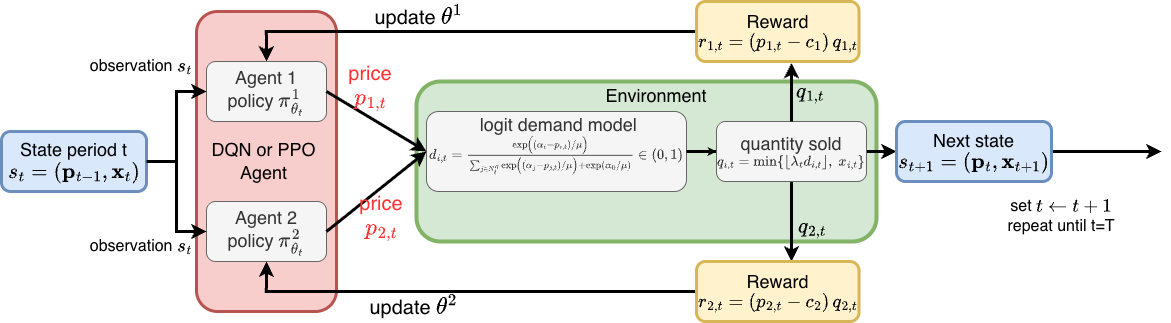
\includegraphics[width=0.95\linewidth]{episodiccollusionmodel2.png}
\caption{Interaction flow in the episodic inventory-constrained market.}
\label{fig:episodic_collusion_model}
\end{figure}

\subsection{Demand Model: MNL with Inventory Availability}
Demand is modeled using a multinomial logit (MNL) choice model.
In this model, the attractiveness of each firm is given by $\exp((q_i-p_{i,t})/\mu)$ as a function of quality $q_i$ and price $p_{i,t}$, and demand is allocated according to the relative magnitudes of these terms.
The parameter $\mu>0$ represents the degree of horizontal differentiation, that is, the scale of sensitivity to price differences.

To include the outside option (not purchasing) and allow demand from sold-out firms to be substituted to other firms, we include in the denominator only the set of firms with remaining inventory, $\mathcal{N}_t^{a}:=\{\,j\in\{1,\dots,N\}\mid I_{j,t}>0\,\}$.
The demand share (normalized demand) of firm $i$, denoted by $s_{i,t}\in(0,1)$, is then defined as
\begin{equation}
s_{i,t}
=
\frac{
\exp\!\left(\frac{q_i - p_{i,t}}{\mu}\right)
}{
\exp\!\left(\frac{q_0}{\mu}\right) + \sum_{j\in\mathcal{N}_t^{a}}\exp\!\left(\frac{q_j - p_{j,t}}{\mu}\right)
}
\label{eq:mnl_share}
\end{equation}
where $q_0$ denotes the quality of the outside option, corresponding to vertical differentiation.

Let $\lambda\in\mathbb{N}$ be the demand-scale factor.
The integer demand quantity is given by
\begin{equation}
d_{i,t}=\left\lfloor \lambda\, s_{i,t} \right\rfloor
\label{eq:scaled_demand_const}
\end{equation}
The actual sales quantity is then limited by the remaining inventory through Eq.~\eqref{eq:inventory_update}.

Thus, demand is proportional to the demand share $s_{i,t}$, and $s_{i,t}$ decreases as the price $p_{i,t}$ increases.

\subsection{Competitive and Collusive Benchmarks and the Collusion Index}
To quantify whether an observed episode (or policy) is competitive or collusive, we define two benchmarks in the space of actions: the competitive benchmark given by the Nash equilibrium and the collusive benchmark given by the monopolistic optimum.
We then define a collusion index on the interval from 0 to 1 to measure how far prices rise above the competitive level.

The competitive benchmark here is not a static price equilibrium defined separately at each time step.
Under inventory constraints, a price chosen in one period affects not only current demand but also future inventory levels and future profits.
Therefore, competition must be viewed as a problem in which each firm chooses the entire price path
\begin{equation}
p_i=(p_{i,1},\dots,p_{i,T})
\label{eq:episode_price_vector}
\end{equation}
at the start of the episode rather than choosing prices independently period by period.
Accordingly, the Nash equilibrium in this paper is defined as a state in which, given the rivals' price paths, no firm can increase its total episode profit by unilaterally changing its own entire price path.
Similarly, the collusive benchmark is defined as the solution that maximizes total profit by jointly choosing the entire set of firms' price paths.
Under the no-discounting setting, Friedrich et al.\cite{friedrich2025learning} showed that both the competitive solution and the joint-profit-maximizing solution can be represented by repeating the same price in every period.
We therefore refer to these repeated benchmark prices as the competitive price $p^N$ and the collusive price $p^M$, respectively, and use the corresponding profits
$R^N_{i,t}$ and $R^M_{i,t}$, computed by applying these prices in each period through Eq.~\eqref{eq:profit_reward}, as the benchmarks for the collusion index.


Specifically, we define the episode-level profit gain of firm $i$ as
\begin{equation}
\Delta_{i,e}
:=
\frac{1}{T}\sum_{t=1}^{T}
\frac{\bar{R}_{i,t}-R^N_{i,t}}{R^M_{i,t}-R^N_{i,t}}
\label{eq:episodic_profit_gain}
\end{equation}
where $\bar{R}_{i,t}$ is the observed (realized) profit, and $R^N_{i,t}$ and $R^M_{i,t}$ are the benchmark profits under the Nash equilibrium (competition) and the monopolistic optimum (collusion), respectively.
Throughout this paper, realized quantities are denoted with bars.
Aggregating $\Delta_{i,e}$ across firms, we define the episode-level collusion index $\Delta_e$ by the generalized mean
\begin{equation}
\Delta_{e}
:=
\left(\frac{1}{N}\sum_{i=1}^{N}\Delta_{i,e}^{\gamma}\right)^{1/\gamma}
\label{eq:collusion_index}
\end{equation}
To preserve interpretability even when $\Delta_{i,e}<0$, in the actual computation we replace $\Delta_{i,e}^{\gamma}$ with $\mathrm{sgn}(\Delta_{i,e})|\Delta_{i,e}|^{\gamma}$.
In the experiments, we use $\gamma=0.5$, which makes the index more sensitive than a simple average to unilateral deviations, that is, situations in which only one firm behaves competitively.
The action space of each firm is given not by continuous prices but by a price grid consisting of 15 discrete prices.
Specifically, the available prices are constructed by equally dividing the interval $[\,p^N-\xi(p^M-p^N),\,p^M+\xi(p^M-p^N)\,]$ into 15 points with $\xi=0.2$, and the action indices corresponding to the competitive and collusive prices are set to $a^N=2$ and $a^M=12$, respectively.

% chapter 3
% ここにあった実験設定Settings of experimentはsection 5に移動しました

% chapter 4
\section{Experimental Design}
\label{sec:method_timevarying_lambda}

We now describe the experimental environment obtained by extending the fixed-demand model to a time-varying-demand setting.
The aim of this extension is to introduce non-stationary demand while preserving, in principle, the benchmark competitive and collusive prices by changing only the temporal allocation of total demand and leaving the overall demand calculation and demand shares intact.
This avoids the need to recompute the Nash benchmark price at every time step and therefore makes it possible to evaluate temporal demand variation within practical computation times.

\subsection{Time-Varying Demand-Scale Factor}
In prior work\cite{friedrich2025learning}, the demand-scale factor $\lambda$ is constant throughout the episode.
In this paper, we extend $\lambda$ to a time-dependent factor $\lambda_t$ to represent settings in which the demand level varies within an episode.
% この拡張では，需要関数の形，在庫更新則，報酬構造はそのまま保ち，需要規模のみを時刻依存にする．
% したがって，固定$\lambda$モデルに対する最小限かつ自然な一般化になっている．

In our model, $\lambda_t>0$ is treated as a positive real number rather than being restricted to integers, and the resulting demand quantity is discretized by a floor function.
Accordingly, the demand quantity is obtained by replacing $\lambda$ in Eq.~\eqref{eq:scaled_demand_const} with $\lambda_t$:
\begin{equation}
d_{i,t}=\left\lfloor \lambda_t\, s_{i,t} \right\rfloor
\label{eq:scaled_demand}
\end{equation}
Sales and inventory updates then follow Eq.~\eqref{eq:inventory_update}.

Despite introducing time variation, this extension has the practical advantage that it does not require recomputing the Nash benchmark price in every period.
Here, the Nash benchmark price refers to the benchmark defined over the episode-level price path in Eq.~\eqref{eq:episode_price_vector}.
% 以下でいう「ナッシュ均衡価格」および「共謀価格」は，前節で導入したエピソード全体の価格系列問題に対応する基準価格$p^N$，$p^M$（無割引設定では各期一定）を指す．
The reason is that, under a continuous-demand approximation, the Nash benchmark price under time-varying demand scale coincides with that of the fixed-demand model.
We explain this argument briefly. Removing the floor function gives the continuous-demand approximation $\tilde d_{i,t}:=\lambda_t s_{i,t}$. Given the rivals' price paths, firm $i$ solves
\begin{align}
\max_{(p_{i,1},\dots,p_{i,T})}\quad
&\sum_{t=1}^{T}(p_{i,t}-c_i)\lambda_t s_{i,t}
\quad
\text{s.t.}\quad
\sum_{t=1}^{T}\lambda_t s_{i,t}\le I_i,\ \ p_{i,t}\ge 0,
\label{eq:timevarying_lambda_relaxed_problem}\\
\mathcal{L}_i
=\;
&\sum_{t=1}^{T}\lambda_t\bigl((p_{i,t}-c_i)-\nu_i\bigr)s_{i,t}
+\nu_i I_i,
\label{eq:timevarying_lambda_lagrangian}
\end{align}
where $\nu_i\ge 0$ is the Lagrange multiplier on the inventory constraint. Because $\lambda_t>0$, for any fixed $\nu_i$ the period-$t$ choice is equivalent to maximizing $((p_{i,t}-c_i)-\nu_i)s_{i,t}$, so $\lambda_t$ itself does not change the ordering of candidate prices. Therefore, under the continuous-demand approximation, $\lambda_t$ does not alter the ranking of prices in each period, and when $\sum_{t=1}^{T}\lambda_t = T\bar{\lambda}$, as in our setting, the Nash benchmark price from the fixed-demand case with $\lambda=\bar{\lambda}$ can be used as a common benchmark.
The same argument applies to the joint-profit-maximization problem, and hence also to the collusive benchmark price.

% 厳密には上記証明は成り立たないので、その補足を次でしている。
In the model actually used in our experiments, however, demand is given by $\lfloor \lambda_t s_{i,t}\rfloor$ as in Eq.~\eqref{eq:scaled_demand}.
Because $\lambda_t$ appears inside the floor function, the invariance described above is not guaranteed in a strict sense.
This discrepancy is a boundary effect induced by discretization and is not the main axis of comparison in this paper.
As a supplementary check, we numerically recomputed the competitive benchmark price for fixed-demand, linear-demand, and exponential-demand scenarios.
The linear-demand case matched the fixed-demand case in every period, and even in the exponential-demand case the maximum deviation from the fixed-demand benchmark was only 0.0007 (approximately 0.04\%).

\if 0

\begin{table}[t]
\centering
\small
\setlength{\tabcolsep}{4pt}
\begin{tabular}{llccccc}
\hline
Condition & Agent & $t=1$ & $t=2$ & $t=3$ & $t=4$ & $t=5$ \\
\hline
Fixed        & 0 & 1.7113 & 1.7113 & 1.7113 & 1.7113 & 1.7113 \\
Fixed        & 1 & 1.7031 & 1.7031 & 1.7031 & 1.7031 & 1.7031 \\
Linear       & 0 & 1.7113 & 1.7113 & 1.7113 & 1.7113 & 1.7113 \\
Linear       & 1 & 1.7031 & 1.7031 & 1.7031 & 1.7031 & 1.7031 \\
Exponential  & 0 & 1.7120 & 1.7112 & 1.7106 & 1.7116 & 1.7112 \\
Exponential  & 1 & 1.7037 & 1.7029 & 1.7024 & 1.7035 & 1.7031 \\
\hline
\end{tabular}
\caption{Nash equilibrium prices over five periods under three demand patterns. Each entry is the mean over five runs.}
\label{tab:nash-price-demand-patterns}
\end{table}

\fi

Accordingly, in this paper we retain the competitive and collusive prices from the fixed-demand case as common benchmarks across all scenarios, and treat temporal variation in $\lambda_t$ primarily as an extension that changes how total demand is allocated across time within an episode.

\subsection{Demand-Scale Scenario Design}
To represent reservation-market demand patterns consistent with the ABCDEF law\cite{ShintaniUmeno2023ABCDEF}, we define the demand-scale factor $\lambda_t$ by the following exponential function:
\begin{equation}
\lambda_t = a\exp(b(t-1))
\label{eq:lambda_exp}
\end{equation}

Here, $a>0$ denotes the initial demand scale and $b\in\mathbb{R}$ is the growth-rate parameter.
When $a=1000$ and $b=0$, the environment reduces to the constant-demand case $\lambda_t=1000$, as in prior work.
If $b>0$, demand increases over time; if $b<0$, demand decreases over time.
When the episode length is fixed at 20 steps, the total demand under $a=1000$ and $b=0$ is $\sum_{t=1}^{20} 1000 = 20000$.
By adjusting the pair $(a,b)$ so that the total demand remains equal to this value, we can compare the effect of temporal demand variation on pricing strategies under a common total-demand level.
The relationship between $a$ and $b$ is then given by
\begin{equation}
\sum_{t=1}^{20} a\exp(b(t-1)) = 20000
\label{eq:lambda_sum_constraint}
\end{equation}
Thus, once $a$ is chosen, the value of $b$ is uniquely determined.
Using this relationship, we design increasing-demand and decreasing-demand scenarios and compare the resulting learned pricing behavior.
Specifically, we use the seven values of $a$ shown in Fig.~\ref{fig:visualize_demand_curve}.
Figure~\ref{fig:visualize_demand_curve} visualizes the schedule of the demand-scale factor $\{\lambda_t\}$ obtained by varying the initial demand scale $a$ while maintaining $\sum_{t=1}^{20}\lambda_t=20000$.
Smaller values of $a$ produce increasing-demand scenarios with demand concentrated in the later periods ($b>0$), whereas larger values of $a$ produce decreasing-demand scenarios with demand concentrated in the earlier periods ($b<0$).
When $a=1000$, we obtain $b=0$, corresponding to the constant-demand case.

\begin{figure}[t]
    \centering
    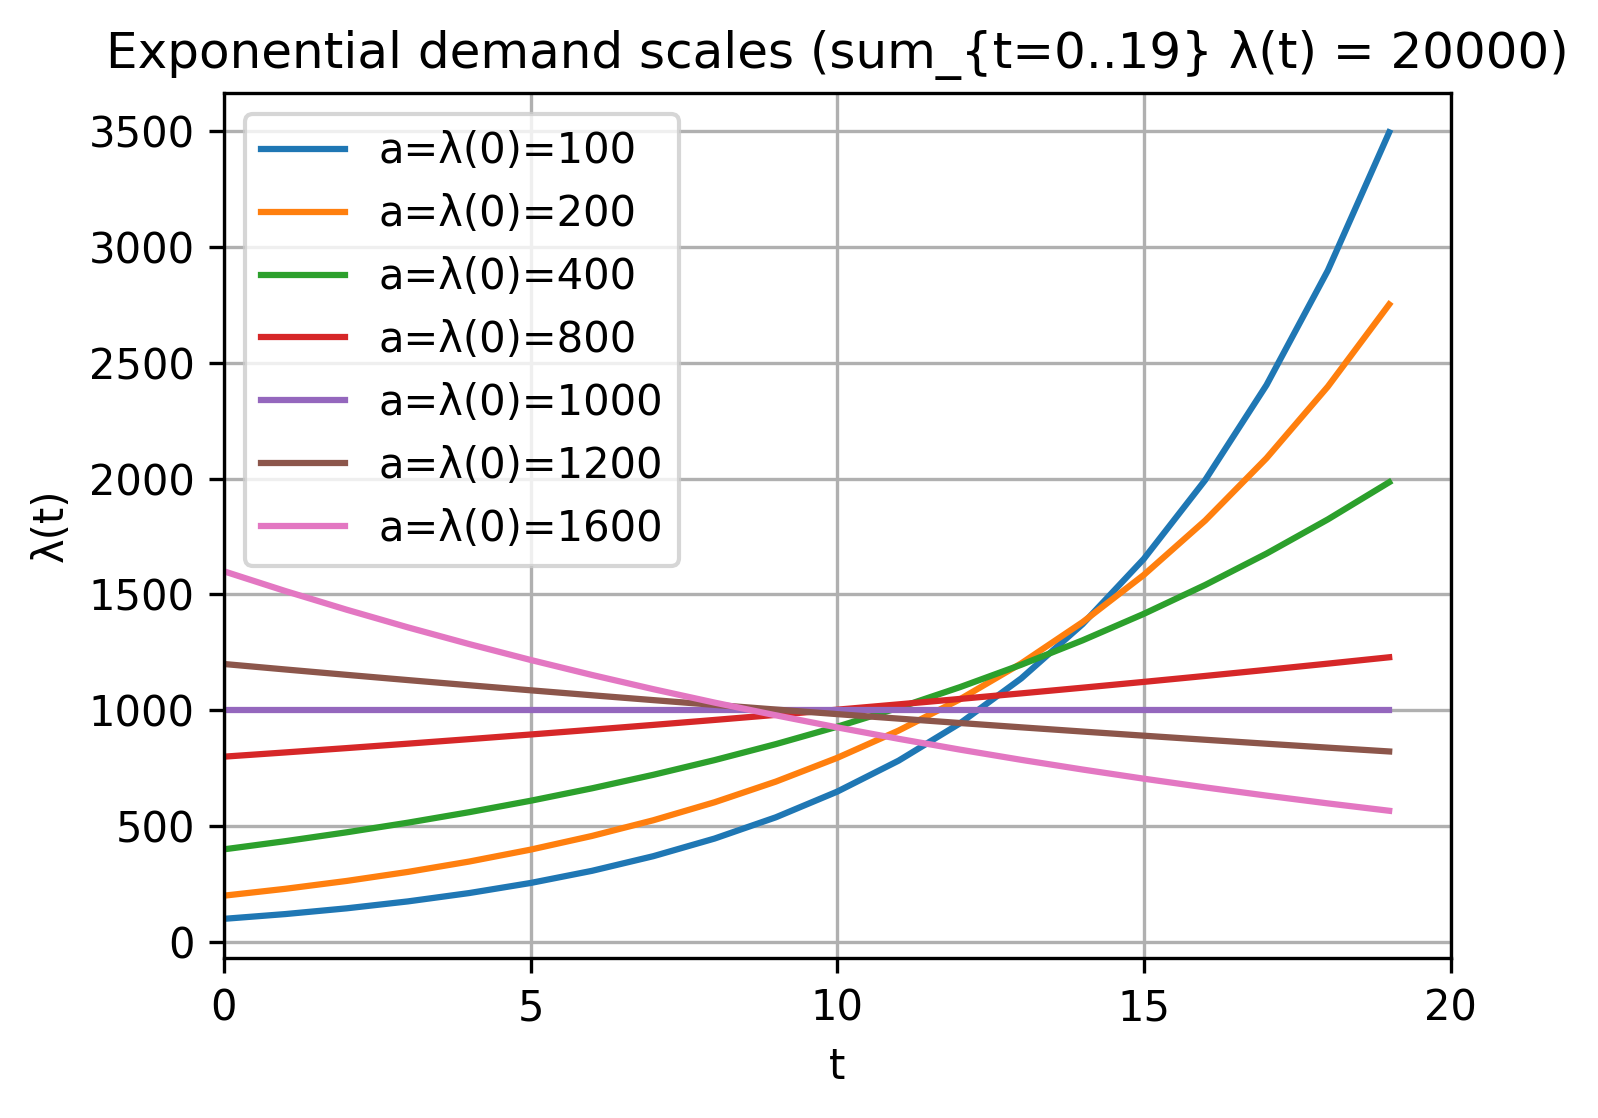
\includegraphics[width=0.7\linewidth]{visualize_demand_curve.png}
    \caption{Exponential demand schedules with equal total demand.}
    \label{fig:visualize_demand_curve}
\end{figure}

In our setting, $\lambda_t$ is not directly observed by the agents.
Instead, agents learn while implicitly inferring the demand level from the time step $t$ and from observed outcomes such as sales and inventory.
This assumption reflects reservation markets in which demand levels vary exogenously and are not fully observable.


\section{Results}

We empirically examine what pricing strategies DQN and PPO learn when the demand-scale factor $\lambda$ is fixed and when it varies over time.

\subsection{Experimental Setup}

We simulate price competition between two firms over episodes of 20 time steps ($t=1, 2, \ldots, 20$).
Each firm learns a pricing strategy using either DQN or PPO.
Unless otherwise stated, the market parameters and the DQN/PPO hyperparameters follow Appendix B.2 (Tables 1--3) of Friedrich et al.\cite{friedrich2025learning}.
The inventory constraint is $I_i=440$ for both agents.
The main modification in this paper is that the demand-scale factor is time-dependent, $\lambda_t$, rather than constant, $\lambda$.
Unless otherwise noted, the learning curves reported below show the mean and standard deviation over 100 random seeds.

\subsection{Learning Dynamics of DQN and PPO}

\subsubsection{Fixed-Demand Environment}

Figure~\ref{fig:algo_compare} overlays the learning dynamics of DQN and PPO in the fixed-demand and time-varying-demand environments using the collusion index.
In the early stage of training, the agents behave exploratorily, and both prices and the collusion index fluctuate substantially.
As training proceeds, prices gradually stabilize.
For both algorithms, the trajectory of the collusion index in the fixed-demand environment is comparable to the result for the fixed-$\lambda$ environment reported by Friedrich et al.\cite{friedrich2025learning}.
The green dashed line in the figure indicates the fully collusive price, and the red dashed line indicates the competitive Nash equilibrium price, showing that the learned strategies lie between these two benchmarks.

\subsubsection{Time-Varying-Demand Environment}

The time-varying condition in the same figure corresponds to an environment in which the demand-scale factor increases exponentially over time according to Eq.~\eqref{eq:lambda_exp}.
Specifically, we set $a=400$, which yields $\lambda_1=400$ at $t=1$ and $\lambda_{20}=1984$ at $t=20$.
Even in the varying-demand condition, the overall pattern of rise and fall in the collusion index is similar to that in the fixed-demand condition.
After the initial exploration period, the prices of both agents converge to approximately 6, and the collusion index stabilizes around 0.28.



\begin{figure}[tb]
\centering
\begin{minipage}[t]{0.48\textwidth}
\centering
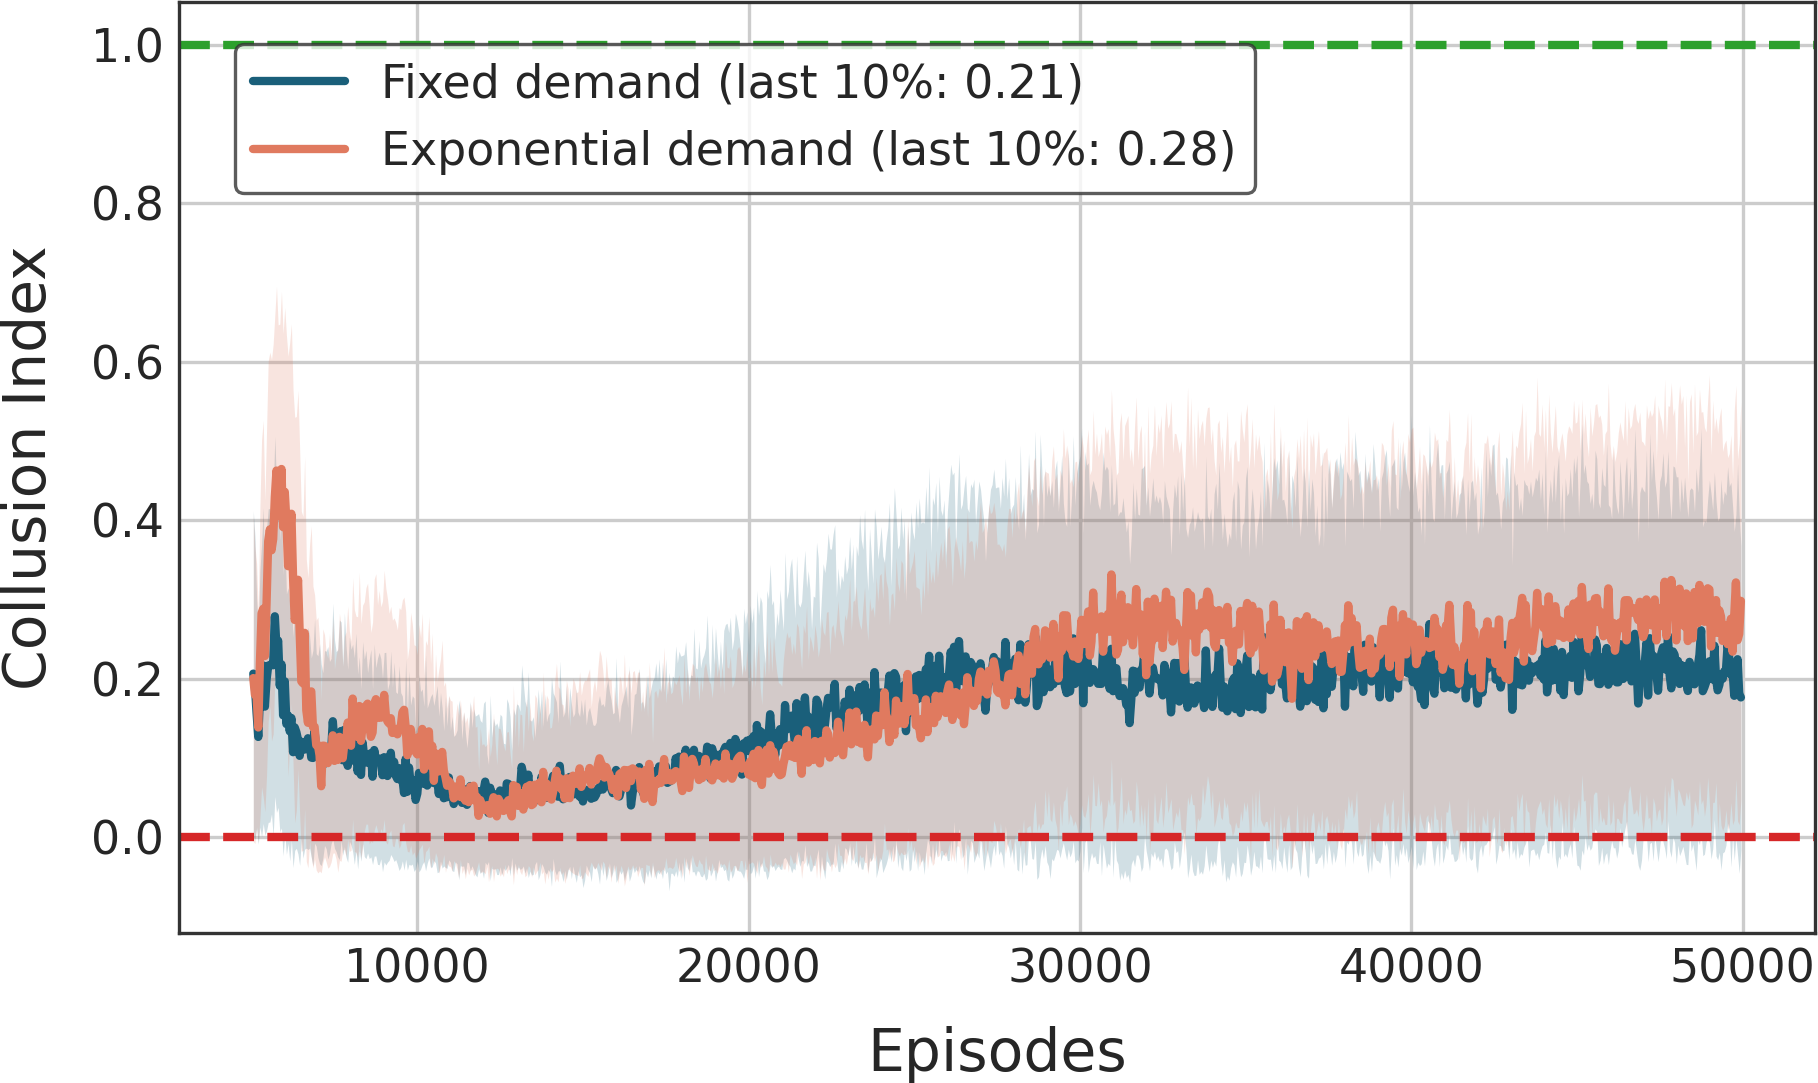
\includegraphics[width=\textwidth]{fig2_DQN_fixed_vs_exponential_collindex_cripped.png}
\end{minipage}
\hfill
\begin{minipage}[t]{0.48\textwidth}
\centering
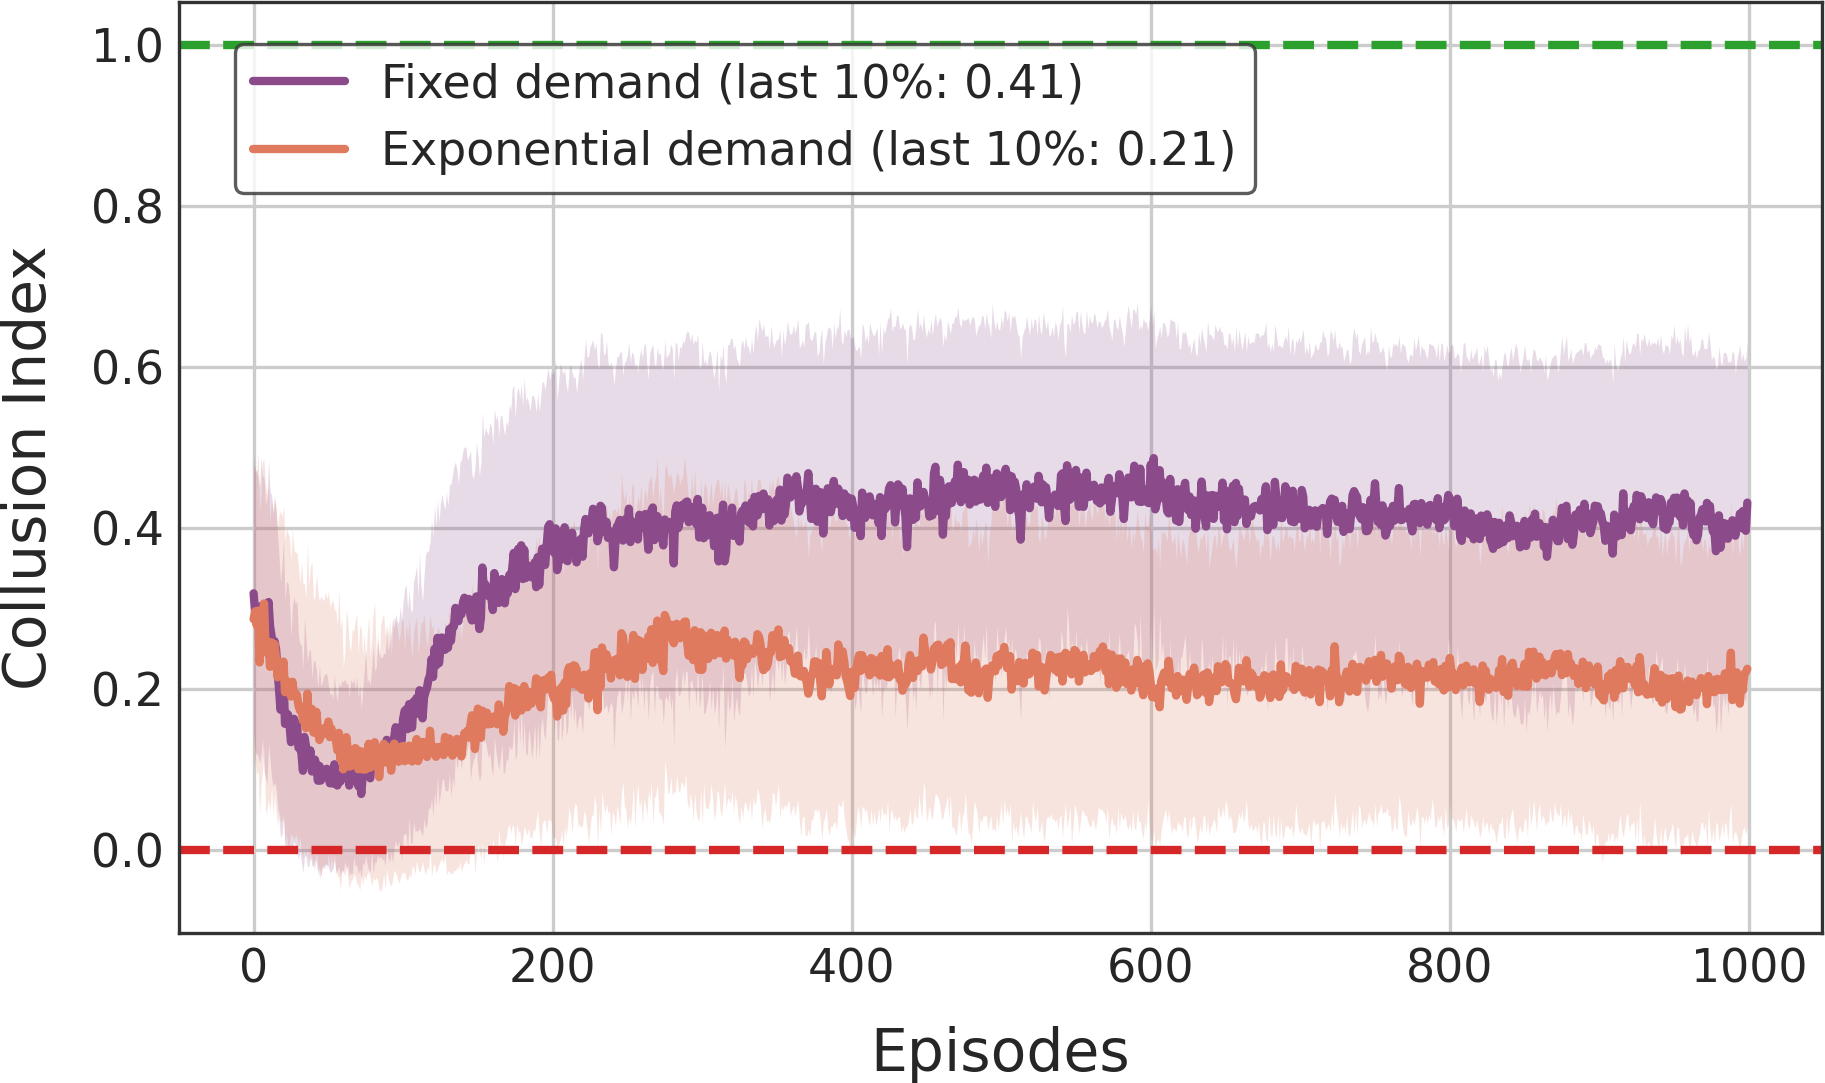
\includegraphics[width=\textwidth]{fig2_PPO_fixed_vs_exponential_collindex_cripped.png}
\end{minipage}
\caption{Comparison of learning dynamics in the fixed-$\lambda$ and time-varying-$\lambda$ environments. Left: DQN. Right: PPO.}
\label{fig:algo_compare}
\end{figure}


Comparing PPO and DQN, DQN is less sensitive to demand variation.
One possible explanation is that DQN updates Q-values from step-level transitions, so the pattern of demand-scale variation over the entire episode may be reflected less directly in per-step decisions.
By contrast, PPO reaches a collusion index of about 0.41 under fixed $\lambda$, but remains around 0.21 under time-varying $\lambda$ (the exponentially increasing pattern in Eq.~\eqref{eq:lambda_exp} with $a=400$).
Because PPO updates policies from episode-level trajectories, the value of coordination in the first half of the episode may be evaluated as relatively small when the reward scale in the early phase (where $\lambda$ is small) is much lower than in the later phase.

\subsection{Behavioral Analysis of Learned Agents}

To examine how the learned policies determine prices within an episode, we inspect evaluation episodes of trained PPO agents, for which the effect of demand variation is particularly pronounced.
Figure~\ref{fig:ppo_eval_episode_compare} shows that, compared with the fixed-$\lambda$ environment, the time-varying-$\lambda$ environment yields lower prices in the initial steps.
The increase in demand scale toward the end of the episode appears to reduce the relative value of collusive behavior in the first half of the episode.

Figure~\ref{fig:ppo_forced_deviation_compare} compares forced-deviation responses in the fixed-$\lambda$ case (left) and the exponentially increasing-$\lambda$ case (right); the upper and lower plots correspond to deviations at $t=1$ and $t=9$, respectively.
In both environments, the other agent adjusts its price after a temporary deviation.
However, in the exponentially increasing-$\lambda$ environment, the price level after returning to collusion is lower than in the fixed-$\lambda$ environment.
This suggests that the lower initial prices do not indicate a collapse into competition; rather, collusion is still present, but at a lower level.

\begin{figure}[tb]
  \centering
  \begin{minipage}[t]{0.48\textwidth}
    \centering
    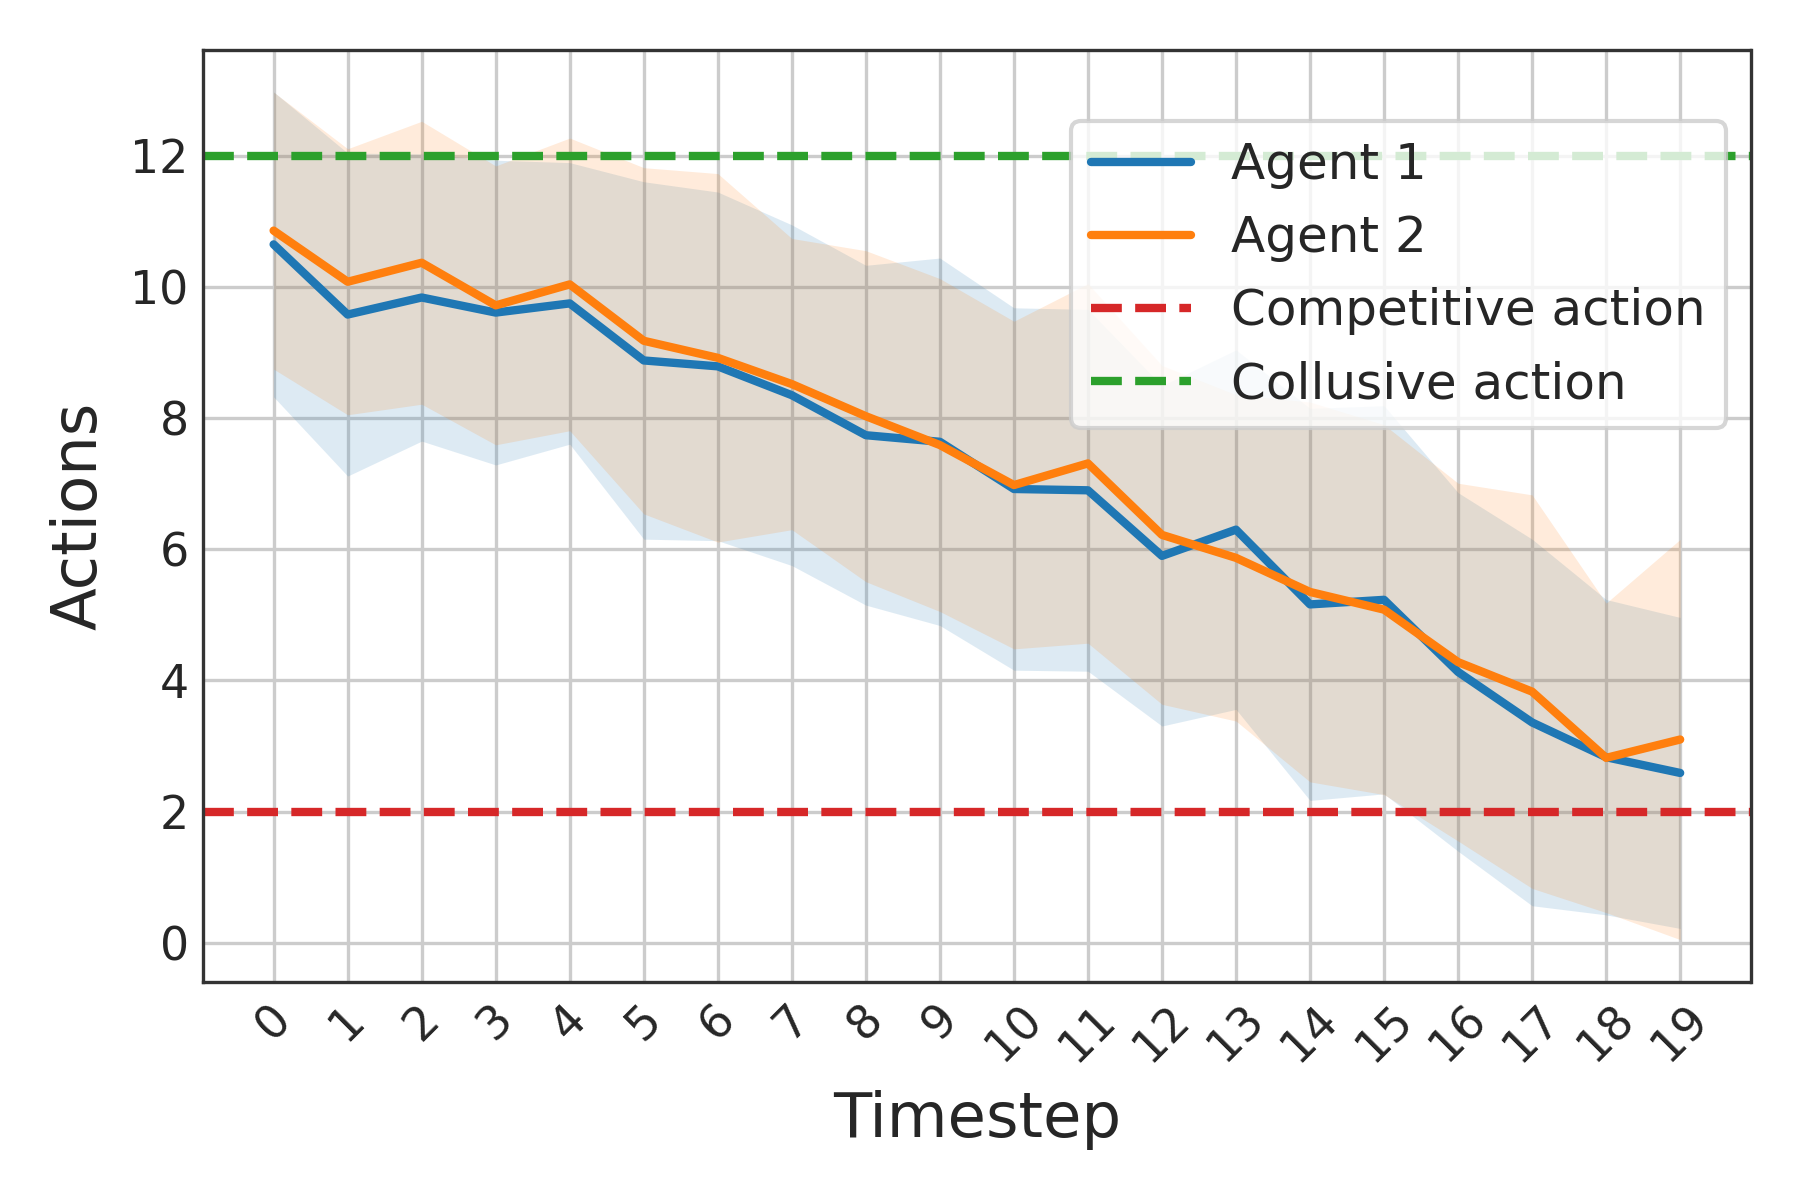
\includegraphics[width=\textwidth]{fig3a_PPO-1000-fixed_evalep.png}
  \end{minipage}
  \hfill
  \begin{minipage}[t]{0.48\textwidth}
    \centering
    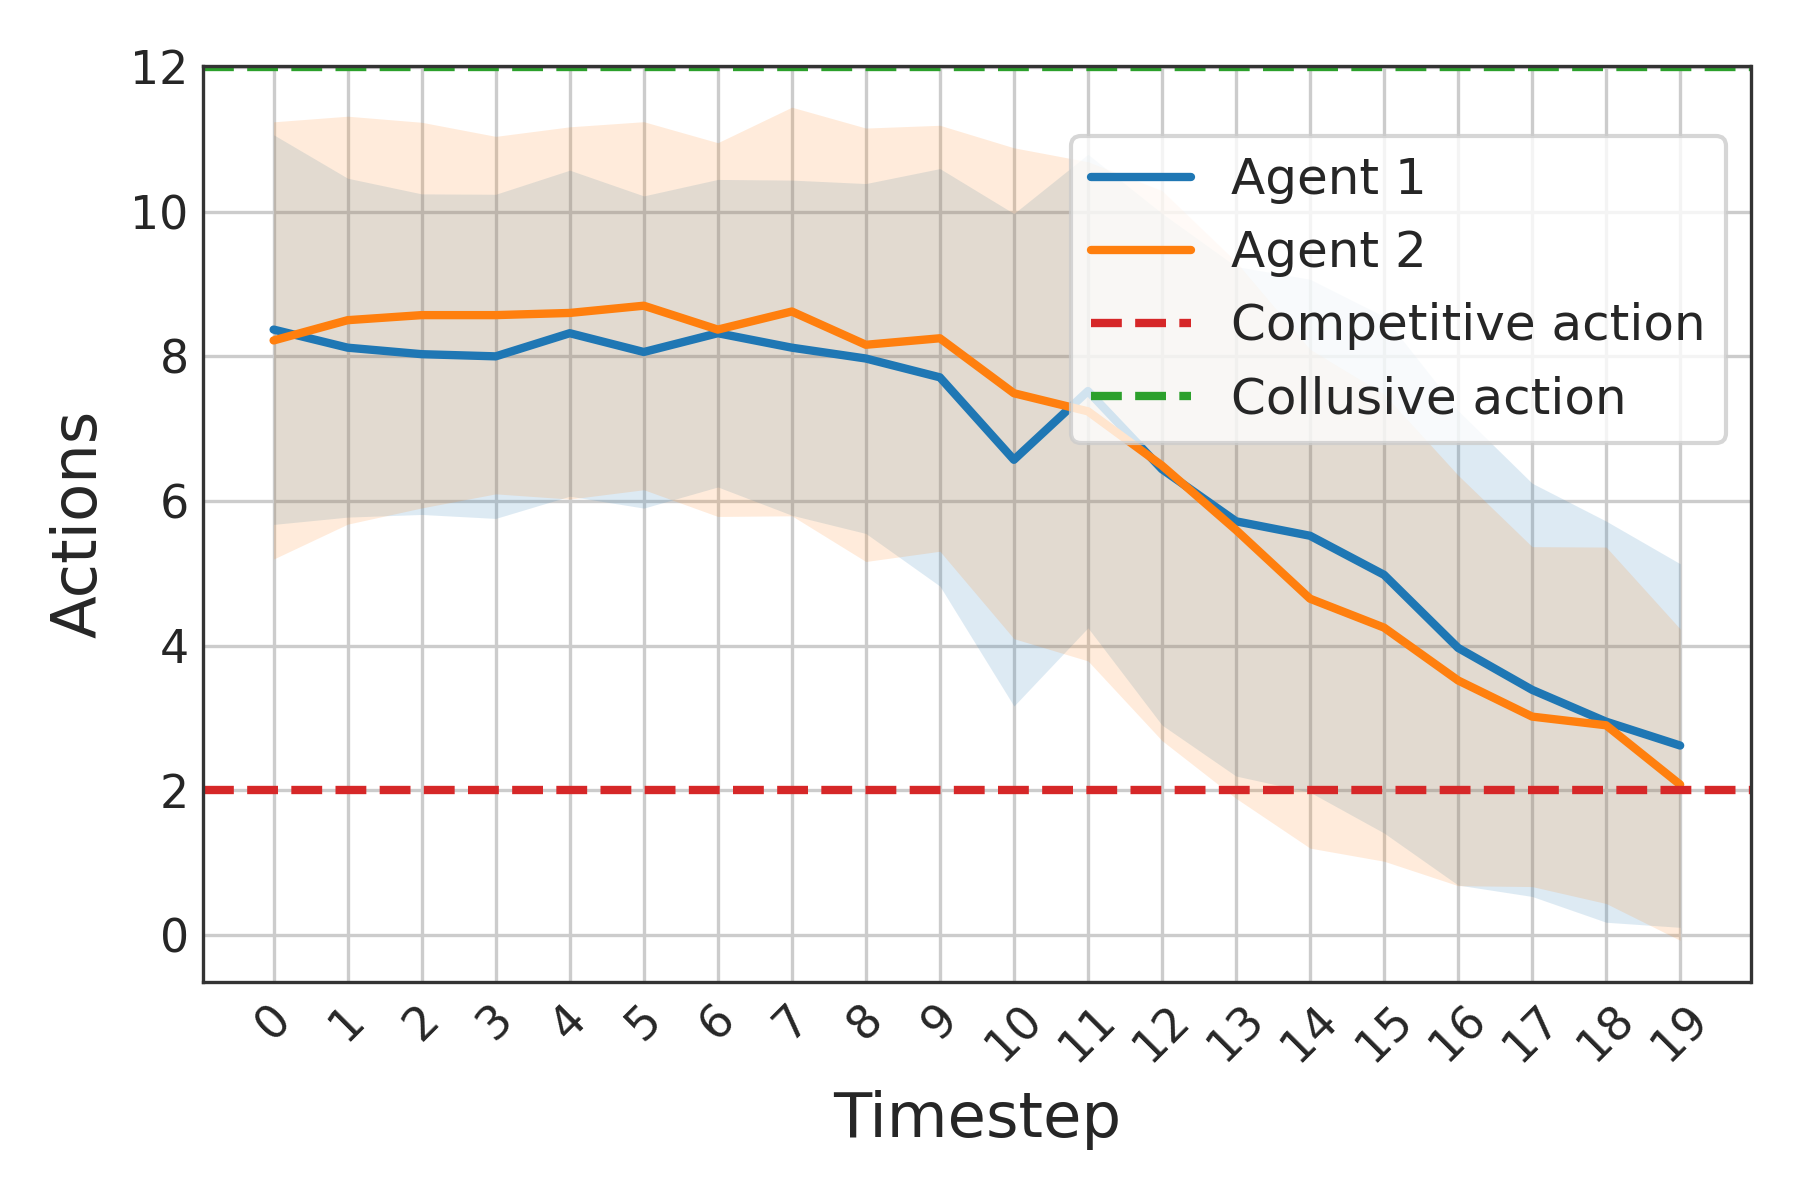
\includegraphics[width=\textwidth]{fig3a_PPO-1000-exponential-400_1984.524399_evalep.png}
  \end{minipage}
  \caption{Comparison of price paths in evaluation episodes of the learned policy. Left: fixed $\lambda$. Right: exponentially increasing $\lambda$.}
  \label{fig:ppo_eval_episode_compare}
\end{figure}

\begin{figure}[tb]
  \centering
  \begin{minipage}[t]{0.48\textwidth}
    \centering
    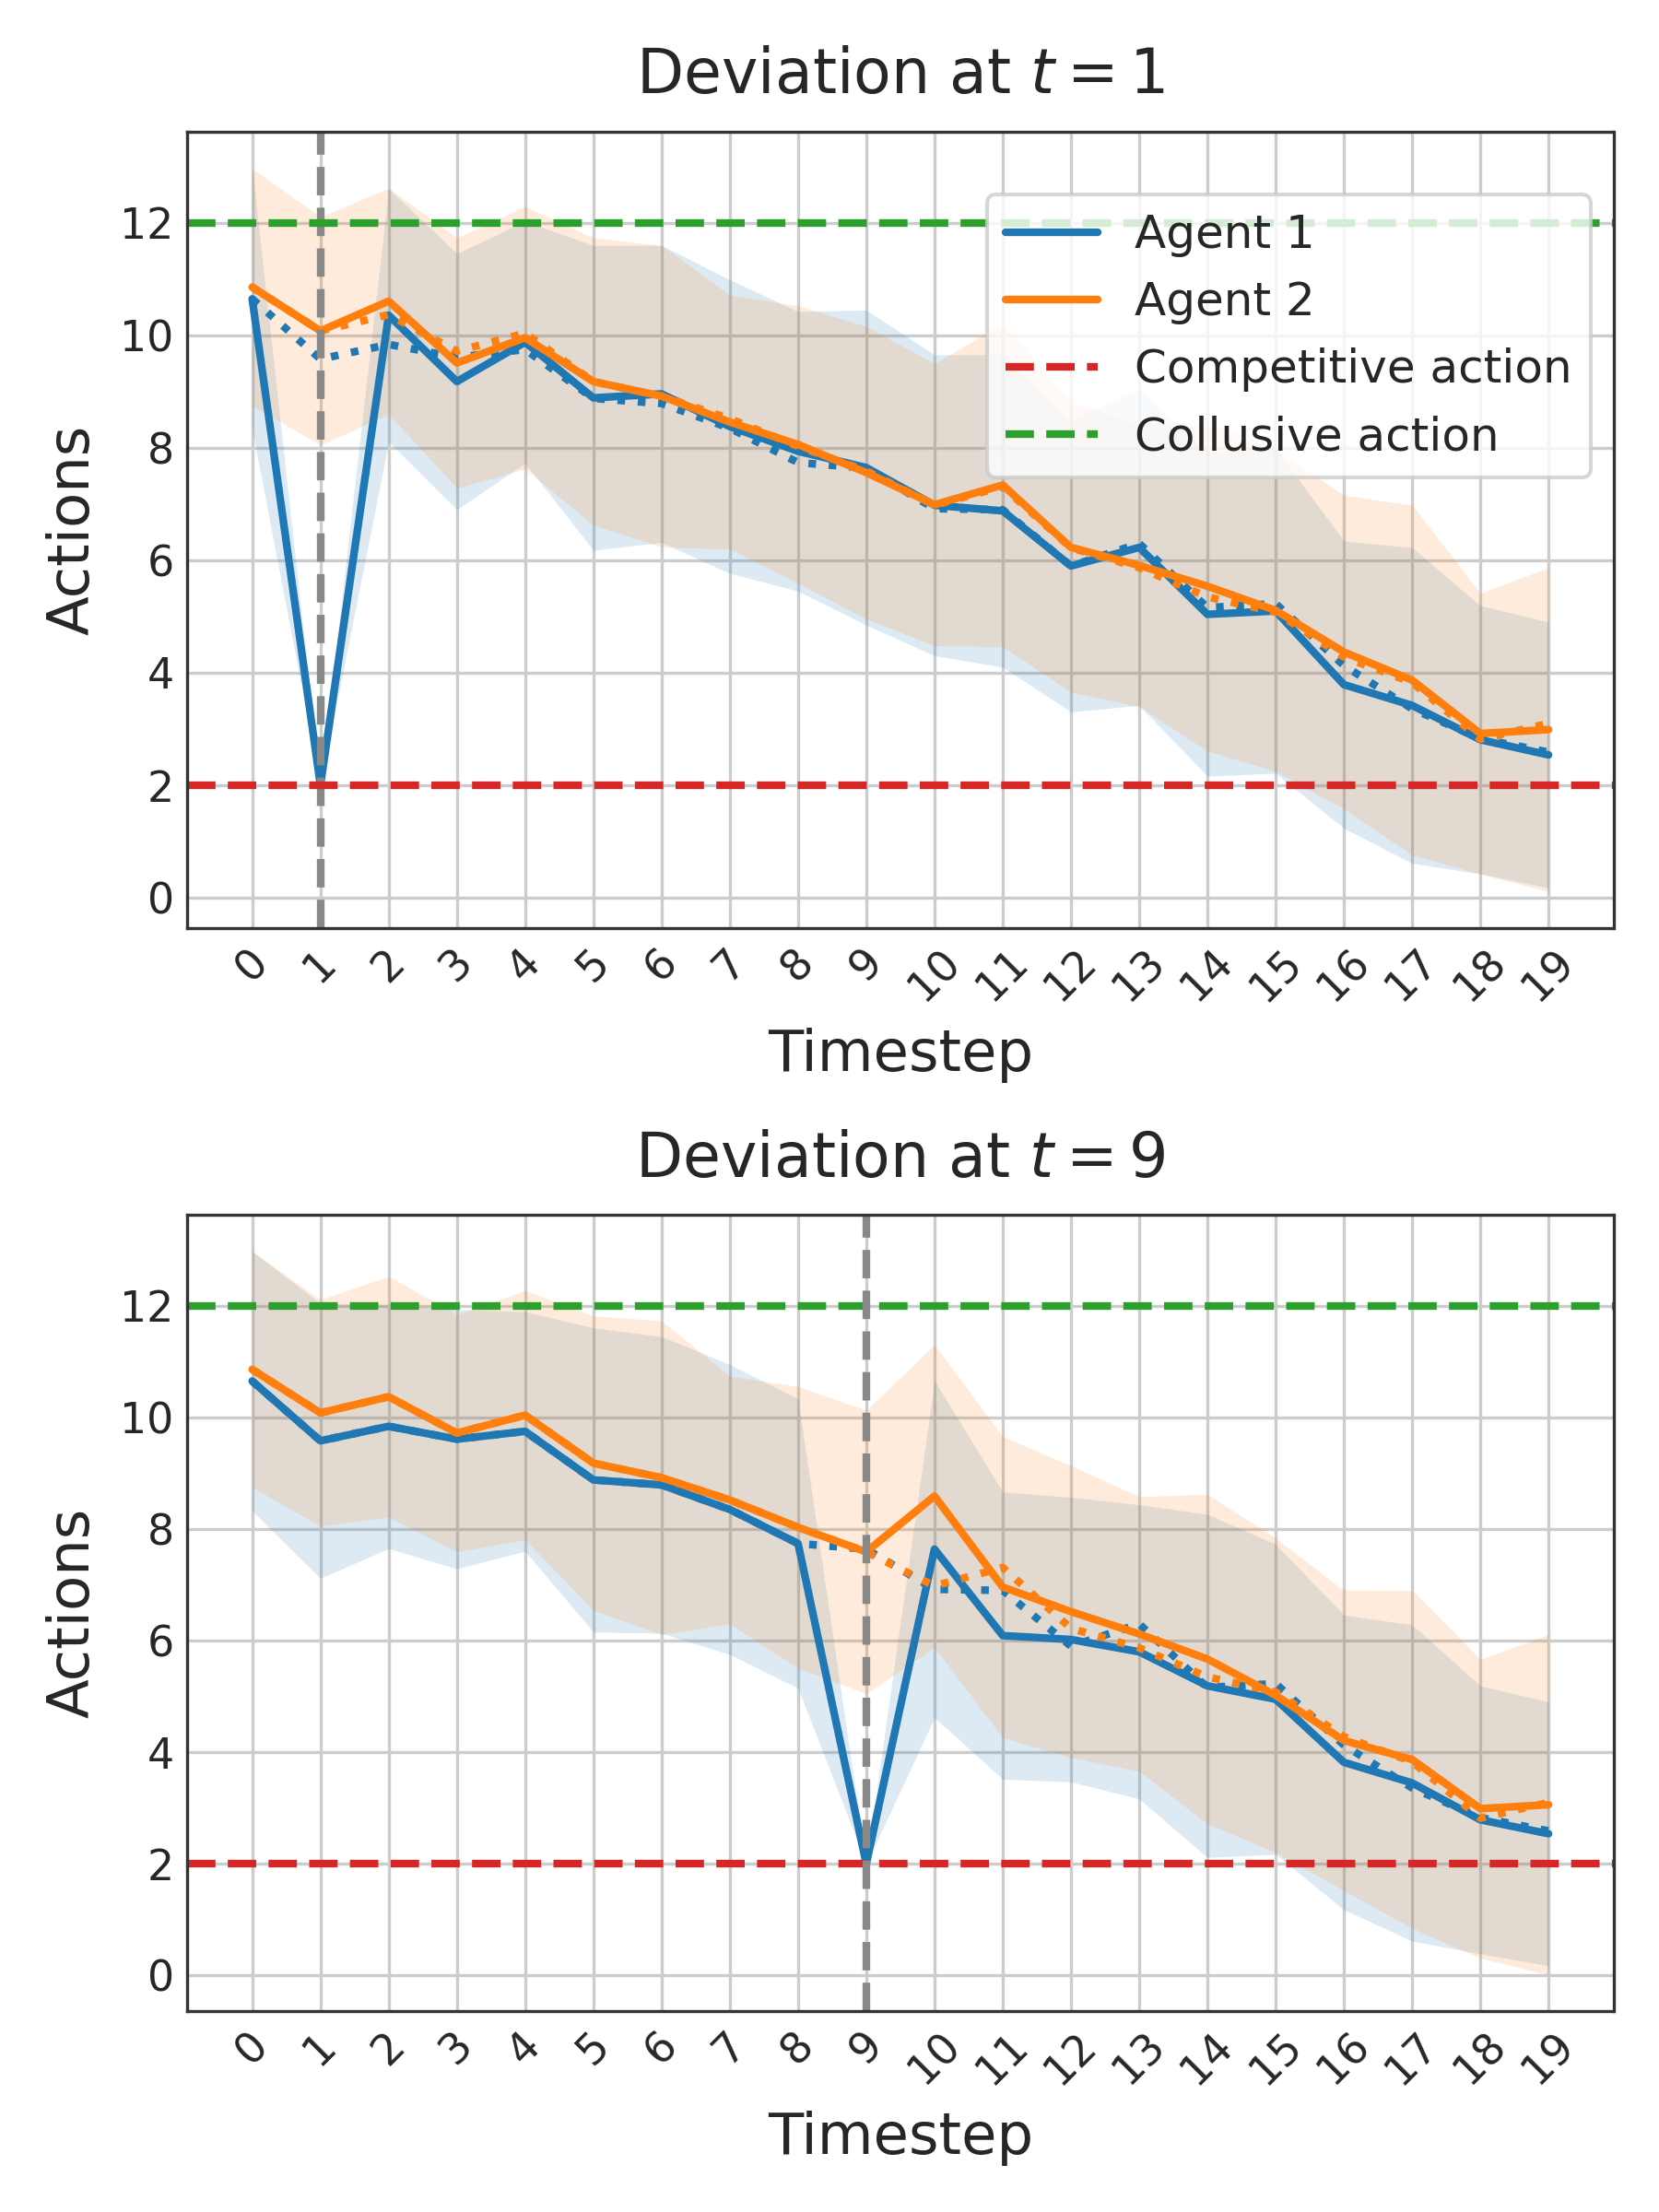
\includegraphics[width=\textwidth]{fig3a_PPO-1000-fixed_forced_dev.png}
  \end{minipage}
  \hfill
  \begin{minipage}[t]{0.48\textwidth}
    \centering
    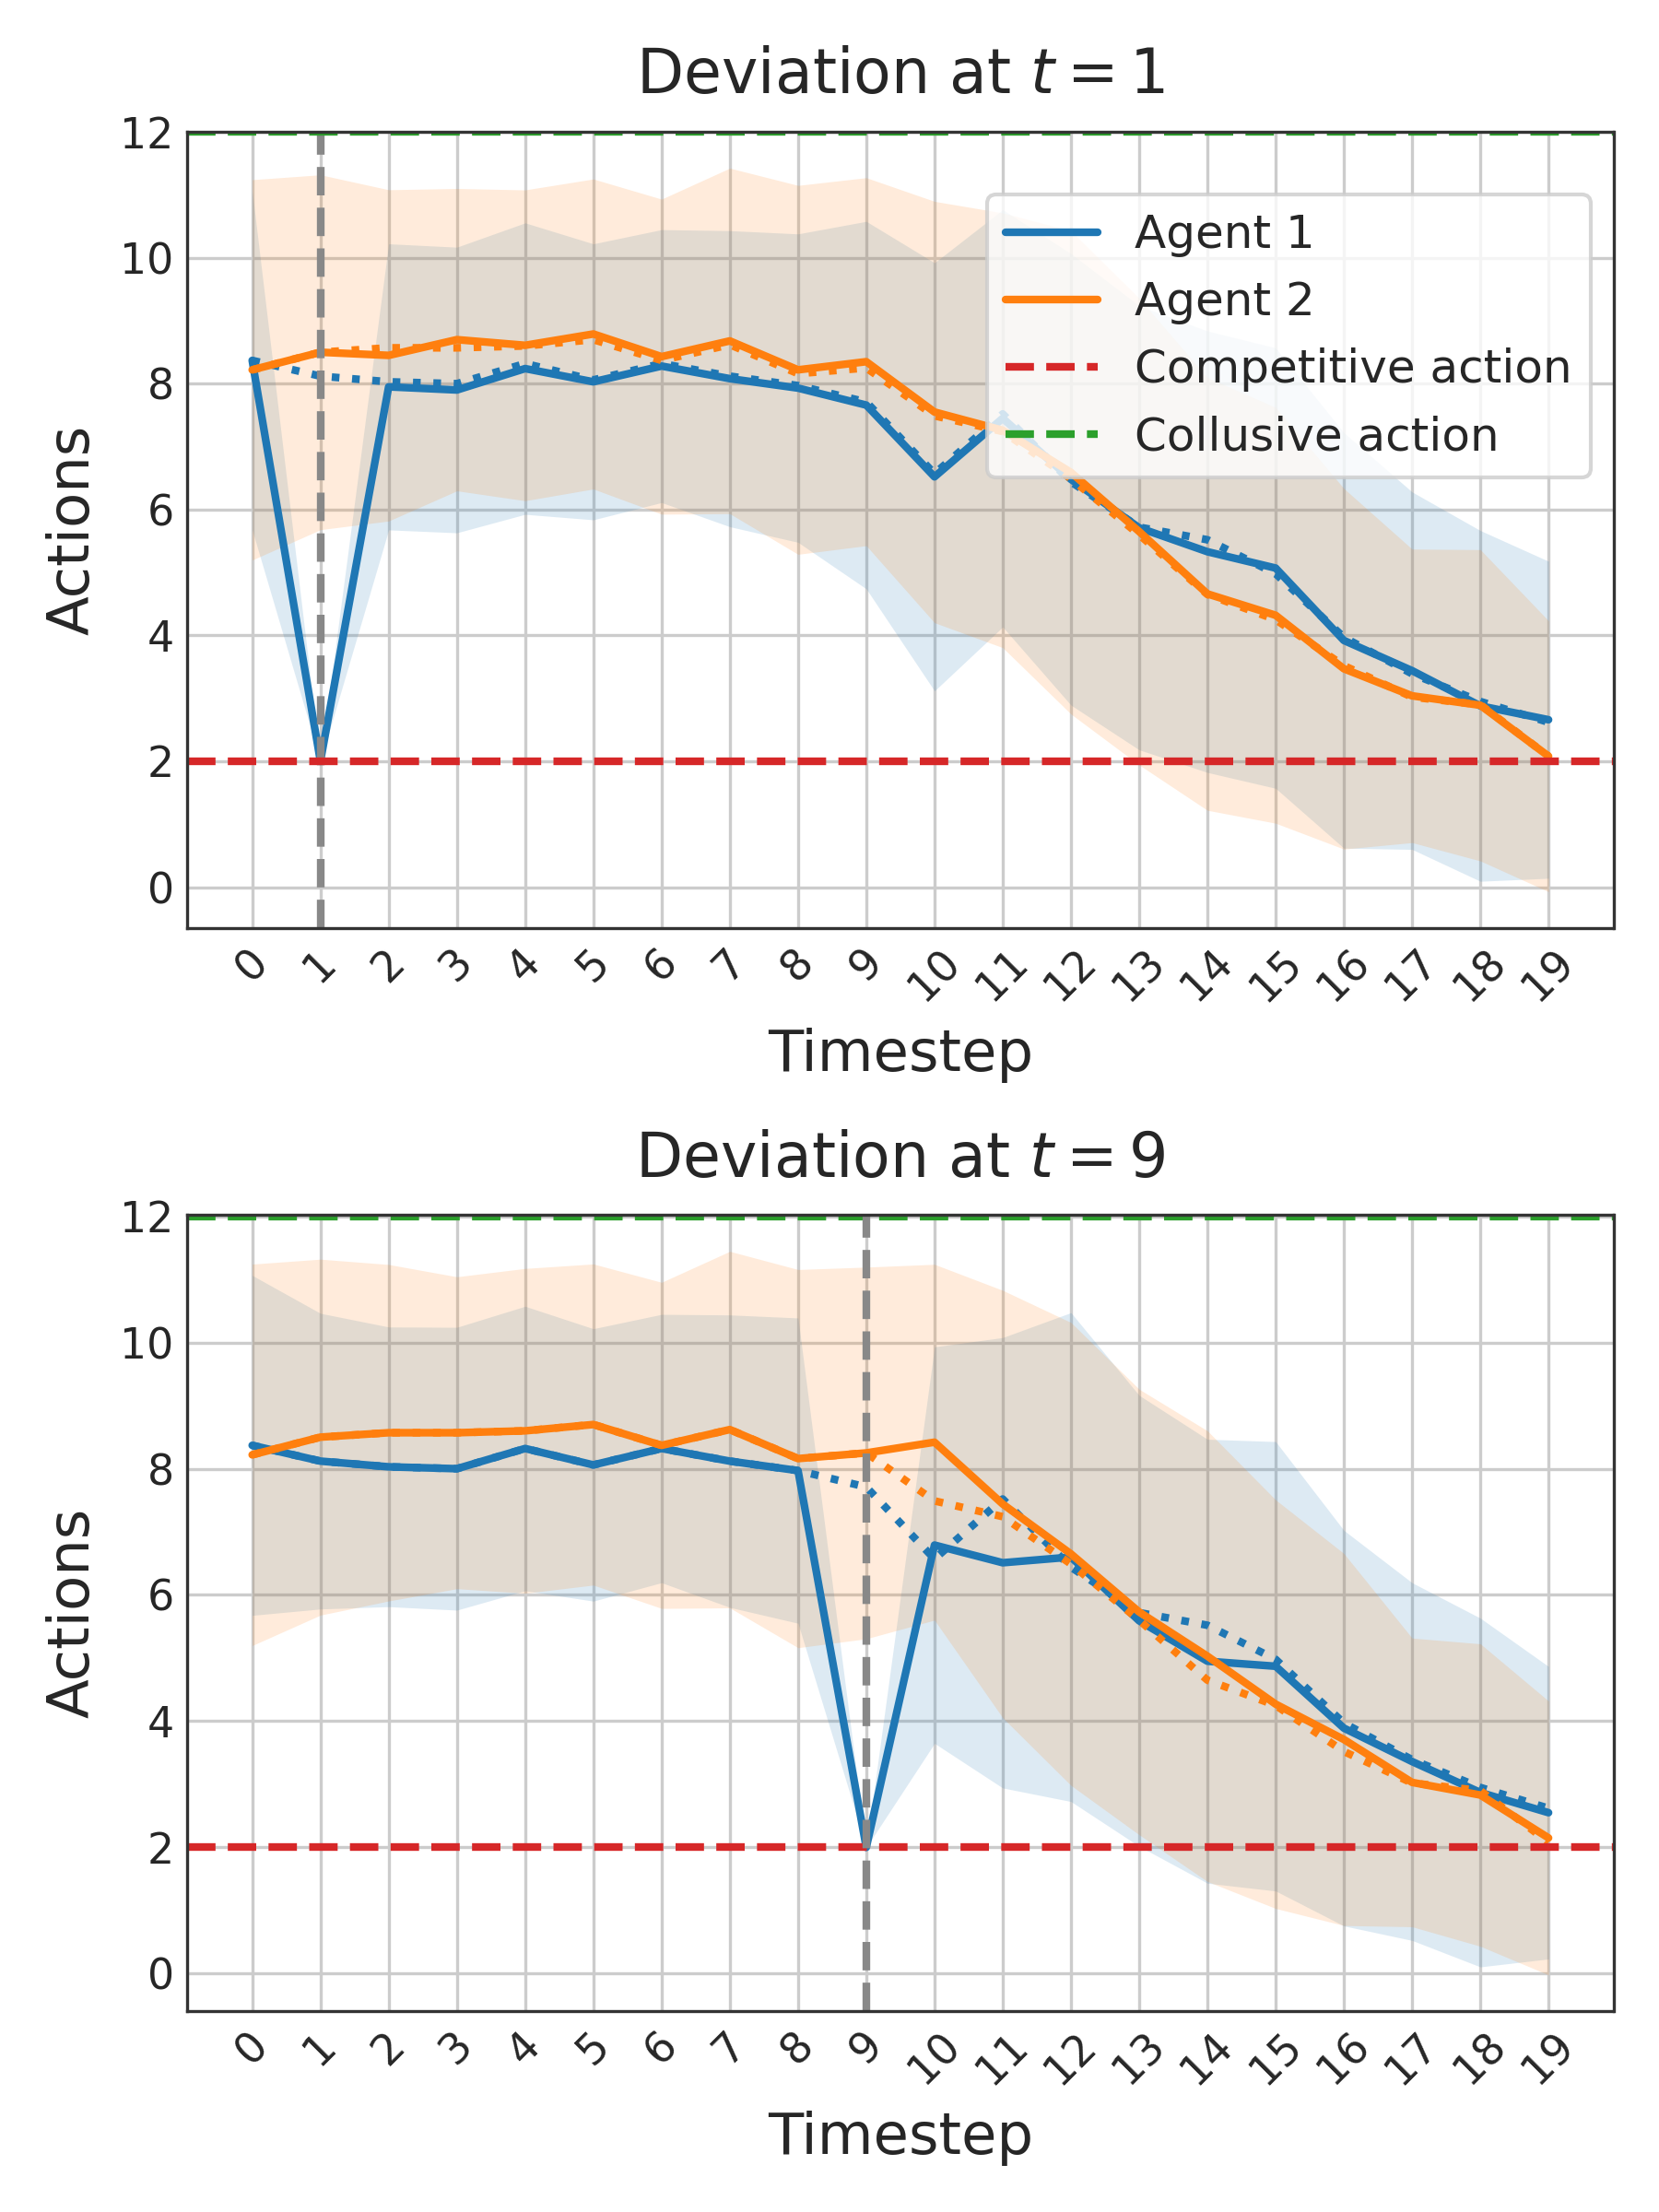
\includegraphics[width=\textwidth]{fig3a_PPO-1000-exponential-400_1984.524399_forced_dev.png}
  \end{minipage}
  \caption{Forced-deviation responses of the learned PPO policy.}
  \label{fig:ppo_forced_deviation_compare}
\end{figure}

\subsection{Rate of Change in Lambda and Converged Collusion}

We next examine how the rate of change in the demand-scale factor $\lambda_t$ under the exponential demand trend in Eq.~\eqref{eq:lambda_exp} affects the converged collusion index.
We consider the seven schedules of the demand-scale factor shown in Fig.~\ref{fig:visualize_demand_curve}, corresponding to $a=100,200,400,800,1000,1200,1600$.
With the episode length fixed at $T=20$, we determine $b$ uniquely for each value of $a$ so that total demand remains constant, as in Eq.~\eqref{eq:lambda_sum_constraint}.

For each condition, we train DQN and PPO with 100 different random seeds.
As the summary statistic for the collusion index, we use the generalized mean with $\gamma=0.5$ defined in Eq.~\eqref{eq:collusion_index}, and compute for each seed the mean over the last 10\% of training.
The results are shown in Table~\ref{tab:ppo_exp_collusion}.

\begin{table}[tb]
\centering
\caption{Collusion index under exponential demand schedules.}
\label{tab:ppo_exp_collusion}
\small
\setlength{\tabcolsep}{4pt}
\begin{tabular}{lrrrrrrr}
\hline
$\lambda_1(=a)$ & 100 & 200 & 400 & 800 & 1000 & 1200 & 1600 \\
$\lfloor \lambda_{20}\rfloor$ & 3494 & 2752 & 1984 & 1228 & 1000 & 822 & 566 \\
Mean CI (DQN) & 0.21 & 0.24 & 0.28 & 0.24 & 0.21 & 0.19 & 0.19 \\
Std.\ CI (DQN) & 0.09 & 0.09 & 0.08 & 0.06 & 0.05 & 0.06 & 0.06 \\
Mean CI (PPO) & 0.14 & 0.16 & 0.21 & 0.30 & 0.41 & 0.48 & 0.55 \\
Std.\ CI (PPO) & 0.13 & 0.09 & 0.12 & 0.10 & 0.13 & 0.15 & 0.19 \\
\hline
\end{tabular}
\end{table}

Table~\ref{tab:ppo_exp_collusion} shows that, for DQN, the collusion index varies only moderately across demand patterns.
For PPO, in contrast, the collusion index tends to be lower in increasing-demand scenarios where demand is concentrated in the later periods, and higher in decreasing-demand scenarios where demand is concentrated in the earlier periods.
The largest difference between the two algorithms appears in the decreasing-demand scenarios with demand concentrated early in the episode ($a=1200,1600$): PPO shows a substantial increase in the collusion index relative to the fixed-demand case, whereas DQN shows a slight decrease.
One possible explanation is that PPO, through on-policy trajectory-based updates, can more easily learn the advantage of maintaining high prices early in the episode when doing so improves total episode profit.
By contrast, DQN relies on off-policy one-step TD learning with a replay buffer, which mixes transitions from high-demand and low-demand periods and may therefore make it more difficult to capture the time-dependent value of inventory allocation.
In scenarios where demand is concentrated in the later periods, the gradients from the later steps may dominate the trajectory-based updates, which may hinder the learning of early-stage coordination and thereby lower the collusion index.
When the inventory constraint is reduced to 420, the qualitative pattern of converged collusion across demand scenarios remains similar, but the overall collusion index becomes lower.
These results suggest that the effect of temporal demand structure on collusion formation is not shared uniformly across learning algorithms, but instead depends on the interaction between the market environment and the learning-update mechanism.


\section{Conclusion and Future Work}

In this paper, we investigated how time-varying demand scale affects the collusive behavior learned by algorithms in episodic inventory-constrained markets.
Our main finding is that the temporal structure of demand has a substantial effect on collusion formation by learning agents.
In particular, under PPO, collusion is stronger when demand is concentrated in the early part of the episode, whereas maintaining collusion becomes more difficult when demand is concentrated in the later part.
Under DQN, by contrast, the response to the same environmental variation is comparatively small, suggesting that the learning style of the algorithm, in particular whether it is on-policy or off-policy, may fundamentally affect how agents adapt to demand variation.

These findings suggest that temporal demand patterns observed in reservation markets are not merely a matter of allocating sales opportunities over time, but may also serve as environmental factors that affect the sustainability of algorithmic collusion.
Real airline-ticket and hotel-booking markets inevitably involve seasonality and temporal demand variation, and such temporal structure may therefore affect competition under algorithmic pricing.

In the experiments conducted here, we fixed other environmental parameters such as the horizontal-differentiation parameter and product quality, and focused on the effect of temporal demand variation.
An important direction for future work is to vary these parameters as well and clarify the combined effect of temporal demand variation and other environmental factors on collusion formation.
In addition, while we motivated exponential demand variation by referring to reservation markets, we did not use empirically calibrated values for the rate of increase.
Future work should construct more realistic market environments by combining realistic assumptions on quality, horizontal differentiation, and inventory constraints, and should then examine the implications of algorithmic collusion for real-world markets.


% ---- Bibliography ----

% BibTeX users should specify bibliography style 'splncs04'.
% References will then be sorted and formatted in the correct style.

\bibliographystyle{splncs04}
\bibliography{main}

\end{document}
